\documentclass{letter}
\usepackage{color}
\usepackage{hyperref}
%\usepackage{tabular}
\usepackage{graphicx}
\usepackage{fancyhdr}

\usepackage[vmargin=1.2in]{geometry}
\signature{Quentin Caudron}
\address{211 Eno Hall \\ Ecology and Evolutionary Biology \\ Princeton University \\ Princeton, NJ, 08544}
\begin{document}

\begin{letter}{}
\opening{Dear Sir or Madam,}

We are delighted that the reviewers found our work interesting, useful, and worthy of publication. We would like to thank them for their constructive comments, which will increase the strength of our paper. Below is a response to their specific questions.






\bigskip
\textbf{Reviewer 1 :}

\textit{The estimated reporting rates vary considerably across time (Fig 2). Sometimes they are larger than 1 (Akureyi) which appears unreasonable. More often, they vary by a factor of 2 over time. Does it make sense that Reykavik has decreasing reporting rate, from 0.7 to 0.4, while most other places have increasing rates?}

The parameter $\rho_t$ is perhaps poorly named. Indeed, in an ideal, homogeneous population, and where demographic information is observed in the same population as the available incidence information, then $1 / \rho_t$ is representative of the reporting rate, inferred from cumulative births and cumulative incidence. This situation is somewhat present in Bornholm, where incidence and demographic information are collected for the same geographical area; $1/\rho_t$ for Bornholm changes fairly smoothly, increasing over time, as might perhaps be expected with an improving medical system. In the other populations in our manuscript, where our demographic information comes from a different geographical region than the time-series of disease incidence, then $\rho_t$ is influenced by this confounding factor. $1/\rho_t$ may be larger than one if, for example, the medical districts (responsible for collecting disease incidence information) covers a larger population than the associated municipality (responsible for collecting demographic information such as births). In this case, $\rho_t$ becomes both a reporting rate and a correcting factor for this geographical discrepancy. It is further worth noting that, due to changing municipal and district borders during the course of the study, $\rho_t$ may be prone to significant changes. We have renamed $\rho_t$ the \textit{observation factor}, and included a few sentences in the text, clarifying that $\rho_t$ should not be interpreted immediately as a reporting rate. 



\bigskip
\textit{If the forecasts of epidemic size are allowed to use a flexibly time-varying reporting rate estimate that may involve knowledge of the size of future epidemics, this could lead to over-fitting of the data. Checking that the conclusions are stable if the reporting rate is estimated to be constant, or perhaps with just a linear trend, is essential.}

Sensitivity analysis to the $\rho_t$ parameter is an important procedure in validating the model. We have included, at the end of this document, the three figures from the manuscript, computed with constant and linear $\rho_t$. Regression parameters for the observed epidemic sizes against predicted final sizes (~as in Figure 3 in the manuscript~) are as follows~:

\begin{center}
\begin{tabular}{rccc}
\textbf{Slope} & Constant $\rho_t$ & Linear $\rho_t$ & In manuscript \\
Bornholm  & 1.19 & 1.08 & 1.07 \\
Faroe Islands & 0.33 & 0.37 & 0.60 \\
Reykjav\'{i}k  & 1.28  & 0.77 & 0.96 \\
Hafnarfj\"{o}rdur  & 1.20 & 1.21 & 1.18 \\
Akureyri  & 0.43  & 0.37 & 0.72 \\
Vestmannaeyjar & 0.74 & 0.81 & 1.23
\end{tabular}



\begin{tabular}{rccc}
\boldmath{$R^2$} & Constant $\rho_t$ & Linear $\rho_t$ & In manuscript \\
Bornholm & 0.83 & 0.76 & 0.76  \\
Faroe Islands & 0.39 & 0.39 & 0.77 \\
Reykjav\'{i}k & 0.79 & 0.60 & 0.64 \\
Hafnarfj\"{o}rdur & 0.90 & 0.90 & 0.88 \\
Akureyri & 0.17 & 0.15 & 0.49 \\
Vestmannaeyjar & 0.60 & 0.51 & 0.76
\end{tabular}
\end{center}

Except in Akureyri, all slopes  of the regression lines with linear $\rho_t$ are closer to $1$ than those with constant $\rho_t$. In all cases, the slopes are closer to $1$ when $\rho_t$ is allowed to vary freely in time. This implies that a (~larger~) consistent bias exists between what is predicted and what actually occurs when $\rho_t$ has a constrained functional form. The coefficients of determination $R^2$ are generally much larger in the difficult regions (Faroe Islands, Akureyri) when the observation factor $\rho_t$ is also allowed to vary freely. For the other regions, however, $R^2$ has similar values regardless of the form that $\rho_t$ takes. With these coefficients of determination lending some aspect of confidence in how true the linear regressions hold, it seems that a less constrained $\rho_t$ yields a less biased estimate with similar linear correlation between what is predicted through the model and what is observed in the data, except in geographies that have strong heterogeneities, such as in the Faroe Islands, where populations are isolated and mixing is restricted; and in Akureyri, where we believe there exists a significant mismatch between municipal and district borders, implying a small overlap between incidence and birth data. As such, we do not believe that a time-varying $\rho_t$ leads to overfitting.


\bigskip
\textit{From Fig 1, it appears as though the rate of introductions may have increased over time. I think this was unmodeled. Is it a concern?}

As the population of the different islands has increased over the course of the study period, introductions have indeed increased over time. Whilst this is not explicitly modelled, introductions are not assumed to be statistically defined (by, say, a Poisson process). Instead, the timing of these introductions is captured by the susceptible reconstruction process, and simulations are conditioned on the first time-point in an epidemic, thereby ensuring that information about introductions is included in the model.







\bigskip
\textit{I struggled to understand the justification for Gaussian process (GP) regression [\dots]. It appears as though the authors want to interpolate rather than put a smooth curve through data points that are supposed to have some measurement uncertainty. Is this right?}

We thank the reviewer for drawing our attention to this part of the text. We have mistakenly left out an important sentence on relaxing Gaussian process regressor trajectories, by providing a ``nugget'' term to the diagonal elements of the covariance matrix. This represents the variance of the input values, and the GP now provide the best linear unbiased predictions without forcing the regressor to pass through the data points, given a certain variance on input values (~and hence, a given smoothness~). Used in this manner, the GP is, as the reviewer describes, a smooth curve passing through points with some measurement uncertainty. We have simplified the parts of the text relating to Gaussian processes, for clarity.

The Gaussian Process regression is used as a method of local regression here. The original TSIR paper by Finkenst\"{a}dt and Grenfell (2000) used a LOWESS regressor, and suggested that splines would be an appropriate alternative. Due to the stepwise nature of the data (~cumulative births are smooth, but cumulative cases, due to the spiky epidemics, occur in sharp jumps~), certain regression methods may lend themselves to better fits than other methods. In this figure, we show fits for Gaussian process, LOWESS, and cubic spline regressors, here for Akureyri. These methods result in very similar regression curves. We note that the GP fit yields a smooth, well-fitting curve everywhere. LOWESS regressors are somewhat less flexible on this type of data, requiring a long correlation length to smooth over the stepwise jumps in the data; this is in conflict with allowing the LOWESS to follow the data more closely. Splines, in turn, can suffer from boundary effects, and require resampling of the curves (~or they would go through every point, which would follow the steplike-form and not yield a smooth curve in the case of this data~). The GP, however, follows a more ideal regression curve, for all geographies, and hence is our preferred method. 

\begin{center}
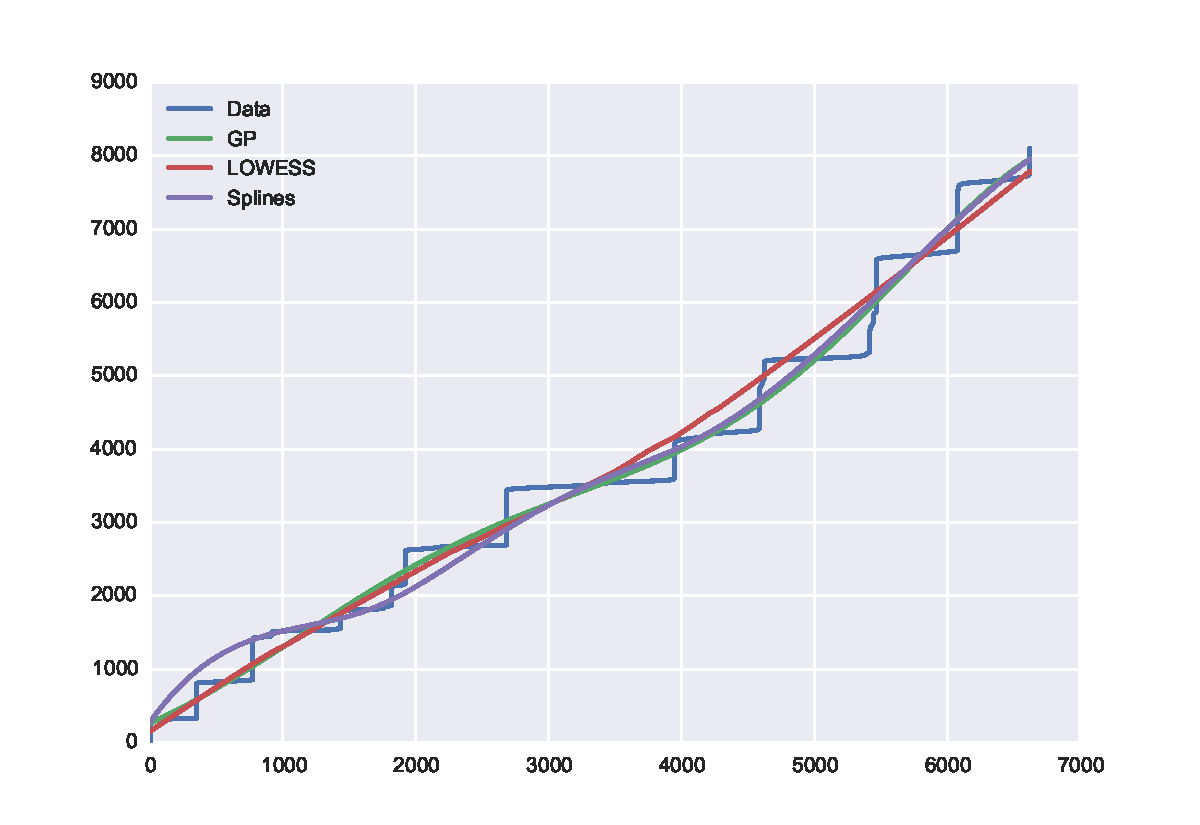
\includegraphics[width=0.8\textwidth]{/users/qcaudron/repositories/SmallPopTSIR/paper/regressors2.pdf}
\end{center}





\bigskip
\textit{The authors appear to suppose that their model has only demographic stochasticity (He et al, 2010). Unless they check that over-dispersion is negligible, there should be an extra dispersion parameter in model equation (6). This will not affect parameter estimates, but may affect forecasts and avoid over-confident confidence intervals.}

We thank the Reviewer for their comment. It is important to check for overdispersion in the model, to avoid invalid statistical fits. He \textit{et al.} (2010) have reported that ignoring environmental stochasticity can lead to biases in parameter estimation. Here, the residuals of our simulations admit a small variance, and hence we believe that overdispersion is negligible. Indeed, when we simulate from an SIR model, fit a TSIR model to the simulated data, and infer its parameters, we are able to retrieve the initial SIR model parameters without bias. As further confirmation, we note that the average slope of the linear regression between predicted and observed final sizes for the six localities comes to $0.96$, very close to the expected, unbiased slope of $1$.









\bigskip
\textit{The TSIR model contains approximations, on top of those of the SEIR model, that are not necessary to fit SEIR models to measles in small communities [\dots]. My suspicion is that the subtle issue of what is lost and gained by moving to the TSIR model can be more trouble than the effort of fitting the SEIR model itself. However, if the goal is forecasting rather than interpreting the fitted model, this distinction becomes less relevant.}

Although the TSIR makes a few additional approximations to the SEIR model, one distinct advantage it has is its computational simplicity. Being extremely quick to implement and computationally cheap to fit, the TSIR model provides a simple and rapid way to infer model parameters, without requiring the use of computationally expensive Monte Carlo methods, as with packages such as \textit{pomp}. Additionally, the TSIR model has been extensively tested on well-mixed populations, but there is little work on applying it to spiky time-series such as those in our dataset. Here, the discrete-time nature of the TSIR model helps greatly in calculating disease dynamics~: continuous-time models such as the SEIR and similar systems of ODEs would require either a statistical model describing importation rates, or a fixed time-series of importations derived from the data, whereas the TSIR encodes these in its reconstruction of the susceptible dynamics. Finally, the TSIR is exceptionally easy to propagate forwards in time, not requiring the use of particle filters or other advanced methods for forecasting.








\bigskip
\textit{It is nice to see that the authors are making the data and code publicly available. Subject to editorial agreement, it might be appropriate to archive this material as supporting files when the paper is published.}

We are happy to continue hosting the complete dataset and code on Github, to remain open-source indefinitely. We are also happy to have the files archived as supporting files, should that be preferable.







\bigskip
\textbf{Reviewer 2 :}

\textit{I think the title might be a little misleading as it seems to me that the approach is predicting the size of an epidemic once started, but cannot predict the timing of epidemics. The timing of future epidemics is a common public health question but is difficult to answer due to the stochastic nature of epidemics in small populations.}

The estimation of epidemic timing is an exceptionally important public health concern; however, as the Reviewer notes, this is a very difficult question to address in small, isolated populations. Over the sixty-five years of data in our dataset, we have not observed more than twelve epidemics for any given locality. This is arguably an insufficient number of data points to fit a statistical model of importation rate, especially noting that epidemics seem to become more frequent in time. Instead, we focus on attempting to predict epidemic size, conditioned only on the first point in any epidemic. In this manner, should we observe a case of measles in a small population today, we may be able to estimate the final size of the epidemic, and hence to inform control measures. However, whilst we have focused on final sizes, we can see from Figure 1 that the duration of epidemics is also relatively well predicted by our model. Nonetheless, we have altered the title to reflect that our focus is on epidemic final size.





\bigskip
\textit{For predicting the sizes of each epidemic/outbreak it is not clear which historical data are required and how long the time-series should be to fit the model in order to make accurate predictions for the size of the next epidemic.}

The historical data required to fit the model are the incidence of disease over time, $C_t$; and the births over time, $B_t$. Obviously, the longer the time-series are, the more predictive power the model may have. We have demonstrated that a significant level of predictability can be had with these time-series, which vary from forty to sixty-five years in length. The amount of data required for a good fit may be significantly less in populations where epidemic data is not so sparse. As we only observe epidemics every three to ten years in these time-series, we only observe a handful of epidemics in total, and so the data contain a smaller amount of information than, say, the time-series of measles in England and Wales used by Finkenst\"{a}dt and Grenfell (2000), where every datapoint contains a non-zero incidence count. We have added a paragraph at the end of the Model Fitting subsection of the manuscript, summarising the general fitting procedure for TSIR models.





\bigskip
\textit{It would be helpful if the authors could clearly state which data are used in this approach: births over time; cases over time; $S_t$? Showing these data in supplementary files would be helpful.}

The TSIR model only required births over time, $B_t$; and observed incidence over time, $C_t$. From these data, the susceptible population over time, $S_t$, can be inferred, along with the observation factor, $\rho_t$. First, the susceptible dynamics $Z_t$ are reconstructed from births and observed incidence; in this process, $\rho_t$ is estimated. The mean susceptible population $\bar{S}$ is then estimated using likelihood profiling, allowing us to compute the susceptible population over time, as $S_t = \bar{S} + Z_t$. We include, as supplementary files, the time-series of observed incidence and births over time, at each locality, and make clear in the manuscript that this is all that is required.




\bigskip
\textit{It is not clear how the birth and case data are used to fit the model. $\rho_t$ looks like it is derived from using data on both births and cases. $r_t$ looks like it is derived from fitting equation (5). Equation (5) includes $I_t$ which is a modelled quantity and does not include $C_t$ which is the time series of observations.}

We appreciate these comments, which have shaped the aforementioned summarising paragraph on fitting the TSIR model at the end of the Fitting section. As specified above, $\rho_t$ is indeed computed from the birth and incidence time-series. $r_t$ is found by likelihood methods during the estimation of $\bar{S}$; they are the maximum likelihood biweekly ``seasonality'' coefficients for fixed $\bar{S}$. Finally, $I_t = \rho_t C_t$ is simply the inferred number of actual cases, that is, the observed number of cases $C_t$ corrected for reporting $r_t$. For a more detailed discussion on the TSIR model, please see Finkenst\"{a}dt and Grenfell (2000), or Reference 13 in the manuscript.







\bigskip
\textit{For $r_t$, this is called the seasonality parameter, but the figures or text do not shed any light on the functional form of this with respect to time.}

The $r_t$ parameter does not have a functional form; it is found by least squares, conditioned on $\bar{S}$. $r_t$ is periodic~: $r_t = r_t+P$, where the period $P$ is one year. As such, the seasonal forcing for an arbitrary period of the year is the same across all years. These coefficients are shown in Figure 2 of the paper, in the right-most column. Estimation of $r_t$ has also been clarified in the summary at the end of the TSIR Model section.






\bigskip
\textit{Could this methodology be modified and applied to the current measles situation in many countries now that vaccination is common leading to irregular and unpredictable outbreaks?}

Vaccination could be encoded into the susceptible reconstruction stage of the TSIR model, where it could appear as a coefficient between 0 and 1 in front of, for example, the births. In this way, the number of individuals entering the susceptible pool would be diminished, mechanistically representing vaccination. This would require a known vaccination coverage, however, as without this, it would not be possible to find $\rho_t$ as a reporting rate. An assumption made in the TSIR model is that all individuals will become infected at some point in their lifetimes. This holds true for all \textit{susceptible} individuals, and thus, representing vaccination as a reduction in the susceptible repletion is possible. However, should we not have the vaccination coverage available, then $\rho_t$ could encompass vaccination rates as well as reporting rates, although these would be impossible to separate without further data. These points are touched upon briefly in the Discussion section.





\bigskip
\textit{Assuming that this approach can be used to predict the size of an epidemic in a small population given some historical data on past epidemics and birth rates, what does this mean for preparedness? What would be the time between the incidence of the first cases, their reports and a model prediction of the size of the outbreak? Could anything be done in this time?}

Given the computational simplicity of this model, predictions could be generated almost immediately after a case were reported. The only data required are the time-series of births and observed disease cases. Conditioned on the availability of these data, this model has the potential for application in informing response, which may differ according to whether a small or large epidemic is predicted. 


\bigskip
We hope that the above points are to the Reviewers� satisfaction, and look forward to hearing from you.



\closing{Yours Faithfully,}



\end{letter}






\pagebreak

\textbf{Constant $\rho_t$~: Reported and predicted biweekly incidence for Bornholm, the Faroe Islands, and four localities in Iceland.}

\includegraphics[width=\textwidth]{/users/qcaudron/repositories/SmallPopTSIR_reviewers/paper/figures_constant/q1.pdf}

\pagebreak


\textbf{Constant $\rho_t$~: Reporting rates and seasonalities.}

\includegraphics[width=\textwidth]{/users/qcaudron/repositories/SmallPopTSIR_reviewers/paper/figures_constant/q2.pdf}

\pagebreak

\textbf{Constant $\rho_t$~: Predictability of epidemic sizes.}

\includegraphics[width=\textwidth]{/users/qcaudron/repositories/SmallPopTSIR_reviewers/paper/figures_constant/q3.pdf}






\pagebreak

\textbf{Linear $\rho_t$~: Reported and predicted biweekly incidence for Bornholm, the Faroe Islands, and four localities in Iceland.}

\includegraphics[width=\textwidth]{/users/qcaudron/repositories/SmallPopTSIR_reviewers/paper/figures_linear/q1.pdf}

\pagebreak


\textbf{Linear $\rho_t$~: Reporting rates and seasonalities.}

\includegraphics[width=\textwidth]{/users/qcaudron/repositories/SmallPopTSIR_reviewers/paper/figures_linear/q2.pdf}

\pagebreak

\textbf{Linear $\rho_t$~: Predictability of epidemic sizes.}

\includegraphics[width=\textwidth]{/users/qcaudron/repositories/SmallPopTSIR_reviewers/paper/figures_linear/q3.pdf}




\end{document}